\documentclass[a4paper,11pt]{article}

\usepackage[toc,page]{appendix}
\usepackage{listings}
\usepackage{appendix}
\usepackage[utf8]{inputenc}
\usepackage[T1]{fontenc}
\usepackage[a4paper,left=2cm,right=2cm,top=2cm,bottom=2cm]{geometry}
\usepackage[english,french]{babel}
\usepackage{fullpage}
\usepackage{setspace}
\usepackage[pdftex]{graphicx}
\usepackage{wrapfig}
\usepackage{soul}
\usepackage{pdflscape}
\usepackage{amsmath}
%\usepackage{ucs}
\usepackage{fancyhdr}
\usepackage{intcalc}
\usepackage{mathastext}
\usepackage{amsthm}
\usepackage{datetime}
\usepackage{xspace}
\usepackage{hyperref}
\usepackage[all]{hypcap}
\usepackage{tikz}
\usepackage{enumerate}
\usepackage{color}
\usepackage{setspace}
\usepackage{here}
\usepackage{titlesec}
\usepackage{pdfpages}
\usepackage{caption}
\usepackage{tcolorbox}
\usepackage{scrextend,rotating}
\usepackage[backend = biber, style = nature, sorting = none]{biblatex}
\addbibresource{biblio.bib}
\usepackage{eurosym}
\usepackage{comment}
\usepackage{framed}
\usepackage{gensymb}
\usepackage{array}

\renewcommand{\appendixpagename}{Annexes}
\renewcommand{\appendixtocname}{Annexes}
 

\hypersetup{colorlinks,citecolor=black,filecolor=black,linkcolor=black,urlcolor=black}

\linespread{1.5}
\AddThinSpaceBeforeFootnotes 
\FrenchFootnotes
\setlength{\parindent}{1cm}
\setlength{\parskip}{1ex plus 0.5ex minus 0.2ex}
\newcommand{\hsp}{\hspace{20pt}}
\newcommand{\HRule}{\rule{\linewidth}{0.5mm}}

\begin{document}

\begin{titlepage}
    \linespread{1}
    	\begin{center}
            \begin{framed}
              \parbox[c][13mm]{215pt}{
                \scriptsize\sf           École polytechnique de Bruxelles\\
                \scriptsize\sf           Bachelier en sciences de l'ingénieur, orientation ingénieur civil\\
                \scriptsize\sf           Deuxième année\\
                \scriptsize\sf           TRAN-H201 - Projet multidisciplinaire II
                }
                \hfill
              \parbox[c][13mm]{178.52396pt}{
\includegraphics[height=13mm]{logo_EPB.jpg}}
            \end{framed}\\[1cm]
            
	%	
\includegraphics[height = 15mm]{logo_EPB.jpg}~\\[1.5cm]
		
		\textsc{\Large Université libre de Bruxelles}\\[1.5cm]
		
		\hrule
		%\begin{framed}
		\begin{framed}{\Large\bfseries \ Projet d'électromécanique - Robot magasinier \\ \huge Rapport de mi-parcours}
		\end{framed}
		%\end{framed}
		\hrule
		
		\vspace{12mm}
		
		\begin{minipage}[t]{0.6\textwidth}
			\begin{center} \large
			\emph{Tuteur :}            \\
			\vspace{2mm}
			Max \textsc{Thulliez}     \\
			\end{center}
		\end{minipage}
		
		\hsp
		
		\begin{minipage}[t]{0.6\textwidth}
			\begin{center} \large
				\emph{Auteurs :}            \\
				\vspace{2mm}
                Loïc \bsc{Dewitte}          \\
                Maxime \bsc{Renard}         \\
                Théo \bsc{Saclier}          \\
                Firas \bsc{Samaan}          \\
                Tristan \bsc{Smeesters}     \\
                Julien \bsc{van Delft}
			\end{center}
		\end{minipage}
			
		\vfill
			
		
\includegraphics[height = 25mm]{sceau.jpg} \\
		\vspace{5mm}
		{\large Belgique \\2019}
	\end{center}
\end{titlepage}
\clearpage

\pagenumbering{roman}
\tableofcontents
%\clearpage
%\pagenumbering{Roman}

%\noindent Nombre de mots du rapport :  \\
%Nombre de caractères de l'abstract :  (espaces non compris)

%\section*{Abstract}
%\section*{But}

\clearpage
\pagenumbering{arabic}

\section{Introduction}

Dans le cadre de leur deuxième année de bachelier à l'École polytechnique de Bruxelles, les étudiants ont été rassemblés par groupe de 6 ou 7 membres afin de réaliser un projet dans la filière de leur choix. Dans la section électromécanique choisie par notre groupe, il s'agit de mettre au point un robot magasinier capable d'effectuer plusieurs tâches définies dans le guide de projet fourni aux étudiants, le tout en moins de deux quadrimestres. Pour ce faire, différents outils sont mis à disposition des groupes de projet: imprimantes 3D, des découpeuses lasers ou encore des machines CNC (computer numerical control). Les composants nécessaires sont quant à eux à déterminer et à se procurer par le groupe, certains par l'intermédiaire de l'École. Ainsi, chaque groupe possède un certain degré de liberté quant à la réalisation et au développement d'un design adapté à la stratégie mise en place pour accomplir la mission imposée.

\section{Description du projet}

\subsection{Objectif}

Concrètement, le robot magasinier devra être capable de déplacer des flacons de diamètre différent : 32, 40 ou 50 mm, depuis leur emplacement jusqu'à une zone de dépôt. Ce processus doit se dérouler en maximum 5min. Ainsi, sur un terrain représentant la configuration d'une usine (voir figure \ref{fig:schéma} ci-dessous), se trouvent trois zones : deux zones de dépôt et une zone de production. Les emplacements sur lesquels seront disposés des flacons au nombre de six se situent sur un parcours préétabli, marqué par de l'autocollant noir. Il en existe trois sortes, de diamètres différents; il y aura donc deux flacons par sorte. Le robot devra ramener deux de ces trois types de flacons dans la zone dédiée à chacun, à savoir une zone pour les flacons de petit diamètre et une pour ceux de grand diamètre. Finalement ceux de tailles moyennes devront rester à leur place respective. Le robot doit compléter entièrement sa tâche en moins de 5 minutes.

\begin{center}
    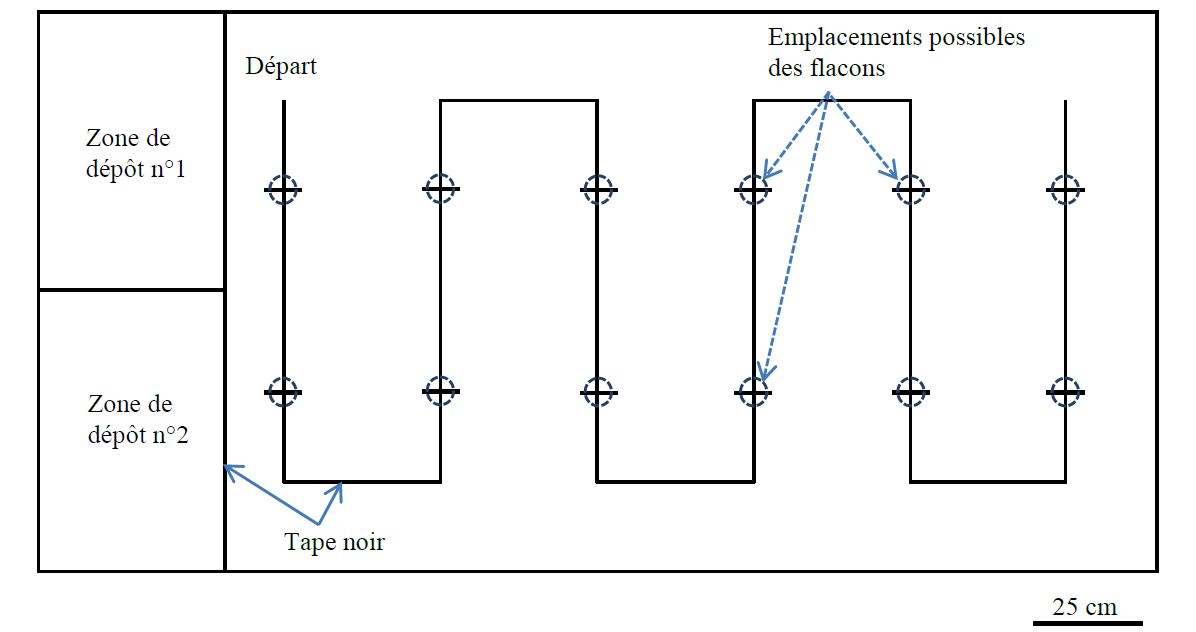
\includegraphics[height=80mm]{schema_circuit.png}
    \captionof{figure}{\label{fig:schéma}Schéma du terrain \cite{cdcharges}}
\end{center}    

Il est demandé aux étudiants de s'occuper de la conception, des plans, de la sélection des composants, de la construction, de la programmation et des tests du robot. Des équipements (Fablab) et formations sont mis à disposition par l'École, complémentés par l'achat de matériel par le groupe. Six tubes en PVC (hauteur = 60mm, Ø = 32, 40 ou 50 mm, 2 de chaque) représenteront les flacons, et ceux de diamètre intermédiaire ne doivent pas être rangés.

\subsection{Contraintes}

Un cahier des charges a pu être dégagé des objectifs et consignes fixées par le guide, imposant dès lors certaines contraintes et limitations.

Ainsi, le budget maximal est de 100 euros. Il doit inclure le coût des composants commandés (par les superviseurs ou pas, à l'exception de la batterie), mais n'intègre pas le matériel récupéré dans le local projet, au Polystock ou à la maison, ni les frais d'utilisation des équipements mis à disposition (imprimantes 3D, découpeuses, etc.).


\section{\label{sec:choix}Choix préliminaires} %(robot dans le rapport final)

Plusieurs idées de fonctionnement du robot (déplacement, préhension, différentiation des tubes, etc.) ont été confrontées avant le choix de fonctionnement actuel, lequel définit le design du robot.

La première concernait un robot suivant le parcours de tape noir, devant mesurer un à un le diamètre des tubes qu'il rencontrerait, les amenant alors à leurs zones attitrées en les attrapant à l'aide d'une pince et en rebroussant chemin, ou les laissant sur place en les soulevant et replaçant une fois passé. Ce mode de fonctionnement semble extrêmement inefficace et lent, amenant moult complications inutiles. De plus, une plate-forme tournante semblait nécessaire au replacement rapide du tube de taille moyenne.

La deuxième proposition impliquait la traversée du parcours au centre de celui-ci (c'est à dire, horizontalement en traversant les lignes verticales sur le plan ci-dessus).
\newline

\begin{figure}[H]
    \centering
    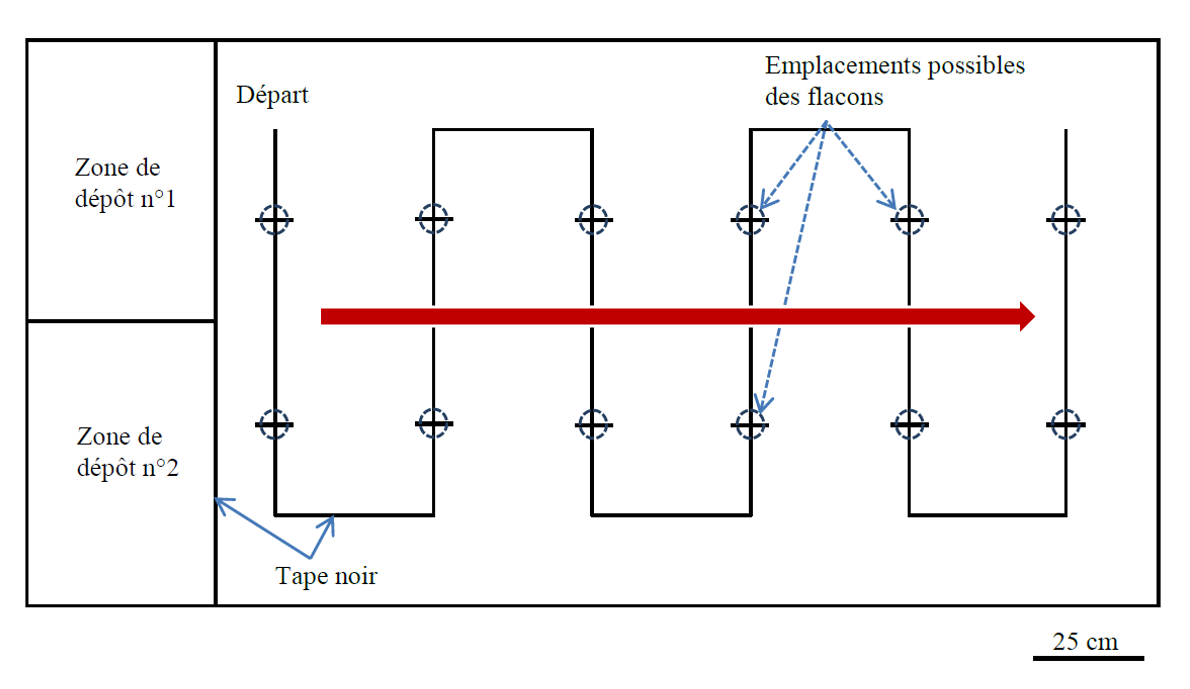
\includegraphics[scale = 0.4]{sens_parcours.PNG}
    \caption{Traversée du parcours}
\end{figure}

En utilisant cette stratégie, deux types de mesures du diamètre des tubes se présentaient : une rotation de 90\degree  suivie d'un déplacement jusqu'au tube, pour qu'une pince mesure mécaniquement son diamètre par le biais d'un servomoteur, ou alors une mesure à distance à l'aide de capteurs infrarouges.

Deux techniques ont été pensées dans le cas où la mesure serait à effectuer à distance. La première impliquait l'utilisation de 3 capteurs infrarouges parallèles pour la mesure d'un seul tube. Selon que ce dernier arbore un diamètre correspondant au petit, moyen ou grand modèle, seraient réfléchis respectivement un, deux ou trois rayons (un par capteur), indiquant le type de flacon en présence duquel est le robot.\\
La seconde s'effectuerait en comptant la durée durant laquelle le tube serait capté par un unique capteur. Le diamètre en serait déduit connaissant la vitesse du véhicule.\\

Le choix s'est porté sur le parcours ne suivant pas le tracé pour des raisons de temps. En effet, le véhicule prendrait beaucoup plus de temps pour faire tout le chemin en suivant l'adhésif. Le temps étant très limité, le premier choix a été préféré. Pour cette même raison, la détection à distance a été privilégiée. Même si cette méthode s'avère légèrement moins précise car victime d'erreurs de détection, le temps reste la priorité car ce dernier est limité à 5 minutes pour la détection et le transport des tubes. De plus, les erreurs de détection peuvent être évitées à l'aide d'intervalles de valeurs plus larges déterminant le diamètre des tubes.

Il a directement été décidé de transporter un tube à la fois, sans en conserver plusieurs simultanément sur le robot. De cette manière, celui-ci pourrait être aisément adapté à une situation similaire où le nombre de tubes changerait. Sa robustesse en cas de changement de configuration en serait ainsi accrue, tout comme sa versatilité. Un système de préhension flexible permettrait également une adaptation à une situation où des tubes de diamètre différent seraient employés. Ainsi, il a semblé nécessaire de trancher entre une pince traditionnelle de face ou attachée à une "grue", venant dès lors attraper les tubes par le dessus. La pince semblait plus simple et sûre, parce que plus basique, répandue et employées, tandis que la "grue" amenait une incertitude quant à la possibilité de glissement du tube, pouvant potentiellement tomber, vaciller ou se positionner de manière oblique, rendant difficile sa pose.

La pince traditionnelle est donc le système de préhension choisi.


\subsection{Microcontrôleur}

Afin de décider quel type de microcontrôleur serait le plus adéquat pour contrôler le robot, il a fallu comparer les différentes possibilités. Parmi les choix adaptés au projet, à sa taille et à son budget (\textit{Raspberry Pi}, \textit{Arduino}), le groupe a opté pour un \textit{Arduino}. Ce dernier est plus facile à manipuler et est suffisant pour les tâches que le protoype devra effectuer, en effet, le robot ne possède pas de caméra, un \textit{Raspberry} n'étant donc pas utile. Bien que celui-ci soit plus puissant, il est surtout plus compliqué. Après avoir envisagé la version \textit{Mega} afin de s'assurer d'avoir un nombre de connexions suffisant, la version \textit{Uno} a été préférée étant donné que le nombre de pins de ce dernier est amplement suffisant aux besoins du véhicule. De plus, l'\textit{Arduino Uno} a été préféré au \textit{Due} car il était limité à un voltage d’opération de 3,3V au lieu de 5V.

\begin{figure}[H]
    \begin{minipage}[c]{.46\linewidth}
    \centering
    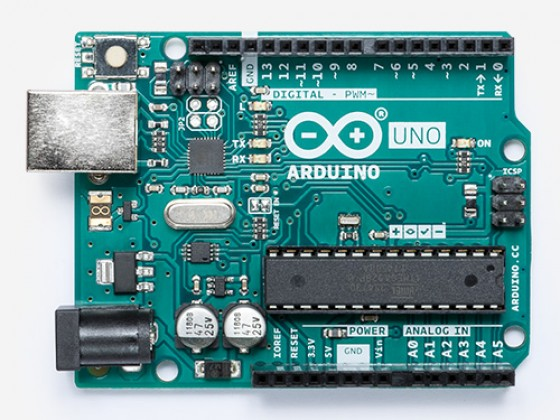
\includegraphics[scale = 0.4]{arduino_uno.jpg}
    \caption{\textit{Arduino Uno} ayant 14 pins digitales et 6 analogiques\cite{arduno}.}
    \label{fig:Uno}
    \end{minipage}
    \hfill
    \begin{minipage}[c]{.46\linewidth}
    \centering
    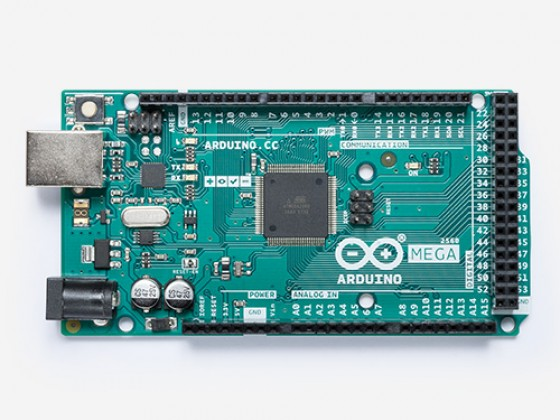
\includegraphics[scale = 0.4]{arduino_mega.jpg}
    \caption{\textit{Arduino Mega} ayant 54 pins digitales et 16 analogiques\cite{ardmega}.}
    \label{fig:Mega}
    \end{minipage}
\end{figure}


\subsection{Véhicule}



Concernant les dimensions de l'appareil, l'environnement dans lequel il évolue suggérait l'utilisation d'un châssis d'un diamètre d'au plus 25 cm, de telle sorte que le véhicule puisse passer entre deux tubes pour rejoindre le centre du terrain après avoir quitté son emplacement de départ. La pince dépassant légèrement du véhicule et par mesure de sécurité, le diamètre décidé est de 17 cm. Il a cependant été indiqué lors de la présentation devant tuteurs que le véhicule pouvait être placé à la guise du groupe avant qu'il ne commence sa tâche, ne devant par conséquent pas débuter son trajet à l'intitulé "Départ" sur le schéma de la Figure \ref{fig:schéma} page \pageref{fig:schéma}. Ces dimensions seront conservées - sauf problème ultérieur - afin de permettre une plus grande liberté de mouvement au robot, et dans l'optique de réutilisation de celui-ci.

Pour le choix des roues, deux possibilités ont été envisagées.L'idée de roues omnidirectionnelles (\ref{fig:mecanum}) a attiré l'attention du groupe pour différentes raisons. Premièrement, celles-ci ont la possibilité de faire se déplacer le robot perpendiculairement au sens traditionnel. Cela aurait permis une grande simplicité dans les déplacements du véhicule, surtout sur un terrain assez cartésien. Le robot aurait pu évoluer librement en se positionnant juste devant une ligne noire et en se déplaçant parallèlement à celle-ci. Toutefois, deux soucis majeurs se présentent avec ces roues : le prix hors budget et la détermination du modèle dynamique afin de concevoir l'odométrie et la régulation.  Il aurait été possible de diminuer les coûts en concevant et imprimant en 3D les roues. De nombreux plans 3D sont disponibles gratuitement sur internet. Toutefois l'incertitude quant au résultat final a suggéré d'écarter cette idée, un des problèmes étant le plastique utilisé pour l'impression ne convenant pas forcément et qui risque d'être trop lisse pour que les roues puissent correctement rouler. Le couple de forces nécessaire pour les mobiliser risquerait d'être trop important dans le cas de frottements trop faibles.

\begin{figure}[H]
    \centering
    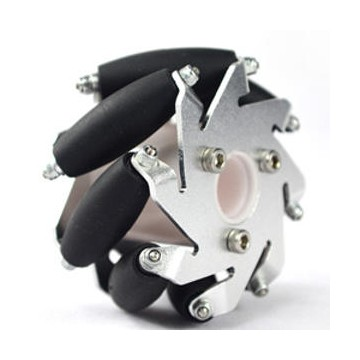
\includegraphics[scale = 0.4]{mecanum.jpg}
    \caption{Roues omnidirectionnelles\cite{mecanum}}
    \label{fig:mecanum}
\end{figure}

Le choix final est un modèle plus simple constitué de deux roues motrices et de deux roues folles. Les roues libres seront des roulettes à bille multidirectionnelles. Elles ont été préférées à de petites roues par soucis de fluidité. Les deux roues motrices sont des roues en silicone de 80mm de diamètre. Celles-si sont munies d'un moyeu de roue en matériau ABS de haute qualité. 

\subsection{Système préhensif}

Comme annoncé précédemment, le groupe a choisi d'employer une pince située à l'avant du véhicule. Le robot ne peut cependant transporter qu'un seul tube à la fois et serait contraint d'effectuer des aller-retours, augmentant le temps requis pour accomplir sa tâche. Ceci est toutefois contrebalancé par la versatilité du robot dont il a été fait mention précédemment, pouvant être adapté aisément à diverses situations. Cependant il est plus efficace lors de la préhension des tubes et s'adapte aisément à tout type de diamètres. Ainsi le robot devrait être capable de terminer toute l'opération dans le temps imparti.

La pince a été modélisée en 3D sur le logiciel \textit{SolidWorks}. Les moteurs ainsi que sa structure principale seront fixés sur l'étage du bas, seuls ses bras dépasseront afin de ne pas agrandir la taille du robot inutilement. Elle doit être capable de se fermer pour attraper les deux tailles différentes de tubes, les bras doivent donc avoir une surface adaptée à la préhension pour une ouverture variable. Afin d'aider cela, cette surface en contact avec les objets sera couverte d'un matériaux caoutchouteux.

\begin{figure}[H]
    \begin{minipage}[c]{.46\linewidth}
        \centering
        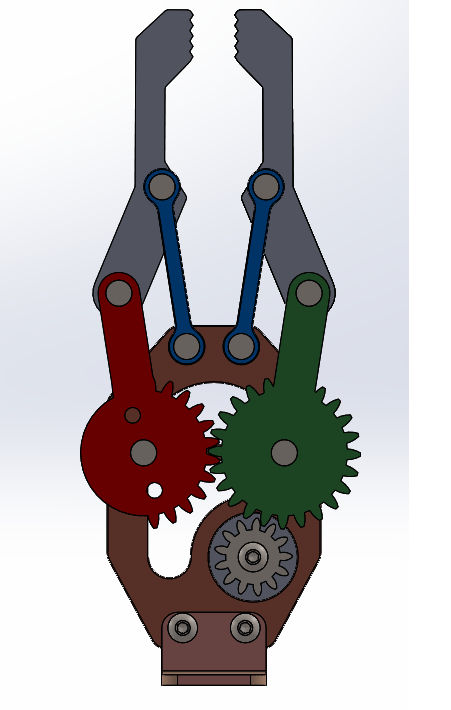
\includegraphics[height = 120]{pince_ferm.png}
        \captionof{figure}{\label{fig:pinceferm}Pince fermée}
    \end{minipage}
    \hfill
    \begin{minipage}[c]{.46\linewidth}
        \centering
        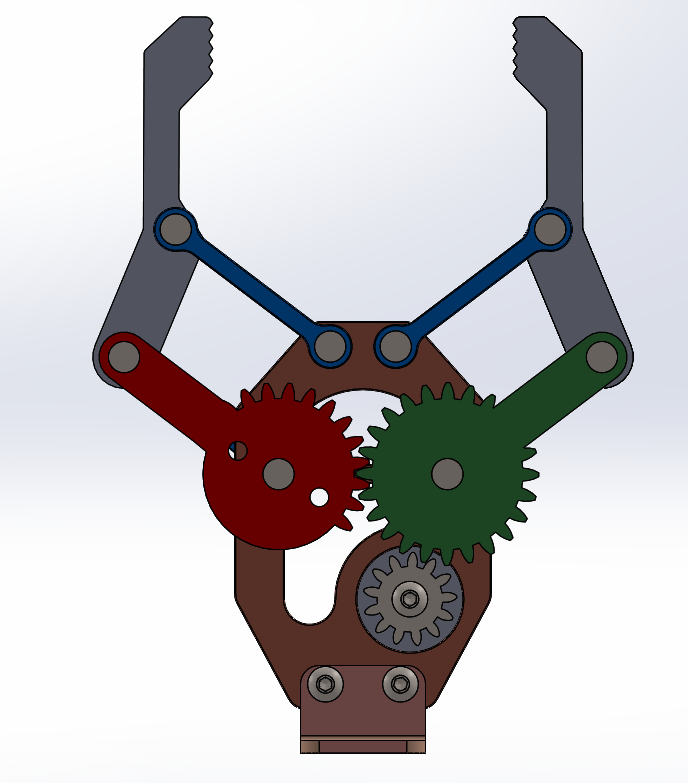
\includegraphics[height = 120]{pince_ouv.png}
        \captionof{figure}{\label{fig:pinceouv}Pince ouverte}
    \end{minipage}
\end{figure}

Pour éviter que les flacons ne frottent sur le sol, la pince devra être munie d'un système élévateur. Un système élévateur vertical avec crémaillère a été envisagé mais rapidement rejeté. Celui-ci apparaît trop complexe et les frottements dus à la crémaillère sont trop importants. Une option plus viable est de fixer directement tout le système de pince sur le moteur placé sur le châssis du bas, la pince se redresse simplement en faisant tourner le moteur. Cela épargne un système élévateur trop complexe et le développement de pièces mécaniques superflues. La pince doit pouvoir se redresser de 90 degrés lorsqu'elle ne transporte pas de tubes. De telle manière qu'en se redressant hors des manoeuvres, la pince n'augmente plus la taille du robot et son diamètre se voit artificiellement réduit. Ainsi les déplacements du véhicules sont facilités. Si possible il est envisagé et probablement réalisable d'augmenter l'angle à plus de 90\degree . De telle façon que la pince puisse même se reposer sur le châssis en dehors des phases de préhension. L'avantage est que de cette manière, les moteurs évitent de travailler excessivement et il n'y aurait pas de forçages des moteurs. Les dimensions exactes de la pince restent encore à définir. Elle serait toutefois munie de 2 moteurs, le premier responsable de sa fermeture et le second dédié au système d'inclinaison.

\subsection{\label{subsec:capteurs}Capteurs}

Le robot possède deux types de capteurs avec deux fonctions totalement différentes, un servant au déplacement du véhicule et l'autre à la détection des tubes.\\
Premièrement, deux capteurs de bord, placés à l'avant du véhicule et orientés vers le bas. Leur rôle est de détecter le tape noir sur le parcours. Le terrain étant principalement de couleur blanche, ces capteurs repèrent assez vite la variation de couleur provoquée par le passage sur un morceau de tape noir. L'un se trouve à droite de la pince et l'autre à sa gauche. Cette disposition est pensée pour parvenir à corriger l'alignement des roues motrices du robot par rapport au tape, voulu parallèle. En effet, le premier capteur à repérer le tape noir enverra un signal à l'Arduino qui diminuera la vitesse de la roue associée au capteur, l'autre roue continuant à tourner jusqu'à ce que le second capteur atteigne le ruban. Le robot peut ensuite continuer à avancer dans une direction perpendiculaire au tape noir.

\begin{figure}[H]
    \centering
    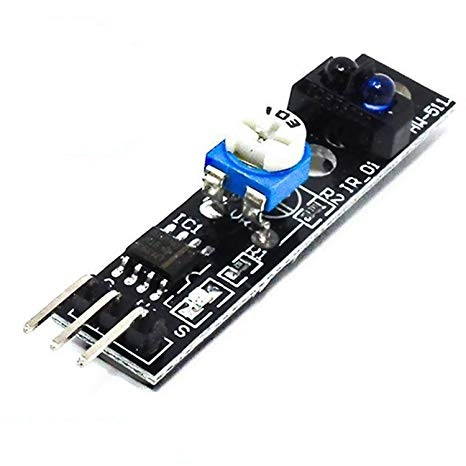
\includegraphics[height = 100]{capteurs.jpg}
    \caption{Capteur de bord : \textit{AZ-Delivery Line follower module}\cite{captbor}}
\end{figure}
\newline

Le second type de capteurs est un capteur à rayons infrarouges. Son rôle est de mesurer le diamètre des différents tubes se trouvant sur le terrain. Un capteur est placé de chaque côté du robot, les rayons émis sont orientés perpendiculairement à la direction d'avancée du robot car sinon il peut y avoir des interférences entres les tubes (l'un entrant dans le cône de détection avant que l'autre en soit sorti comme sur la Figure \ref{fig:cônedetect} ). Ils sont donc placés à la verticale sur le châssis. Les rayons sont donc émis lorsque le véhicule se meut, mais ne sont renvoyés aux capteurs que s'ils ont été réfléchis par un tube. Pendant que le robot avance à vitesse constante relativement faible, la durée de détection des rayons infrarouges est mesurée. Il devient donc trivial de connaître les diamètres des tubes détectés à l'aide de l'équation suivante :
\begin{equation*}
    v . t = d
\end{equation*}
avec v la vitesse du véhicule, t le temps de détection mesuré et d le diamètre du tube

\begin{figure}[H]
    \begin{minipage}[c]{.46\linewidth}
    \centering
    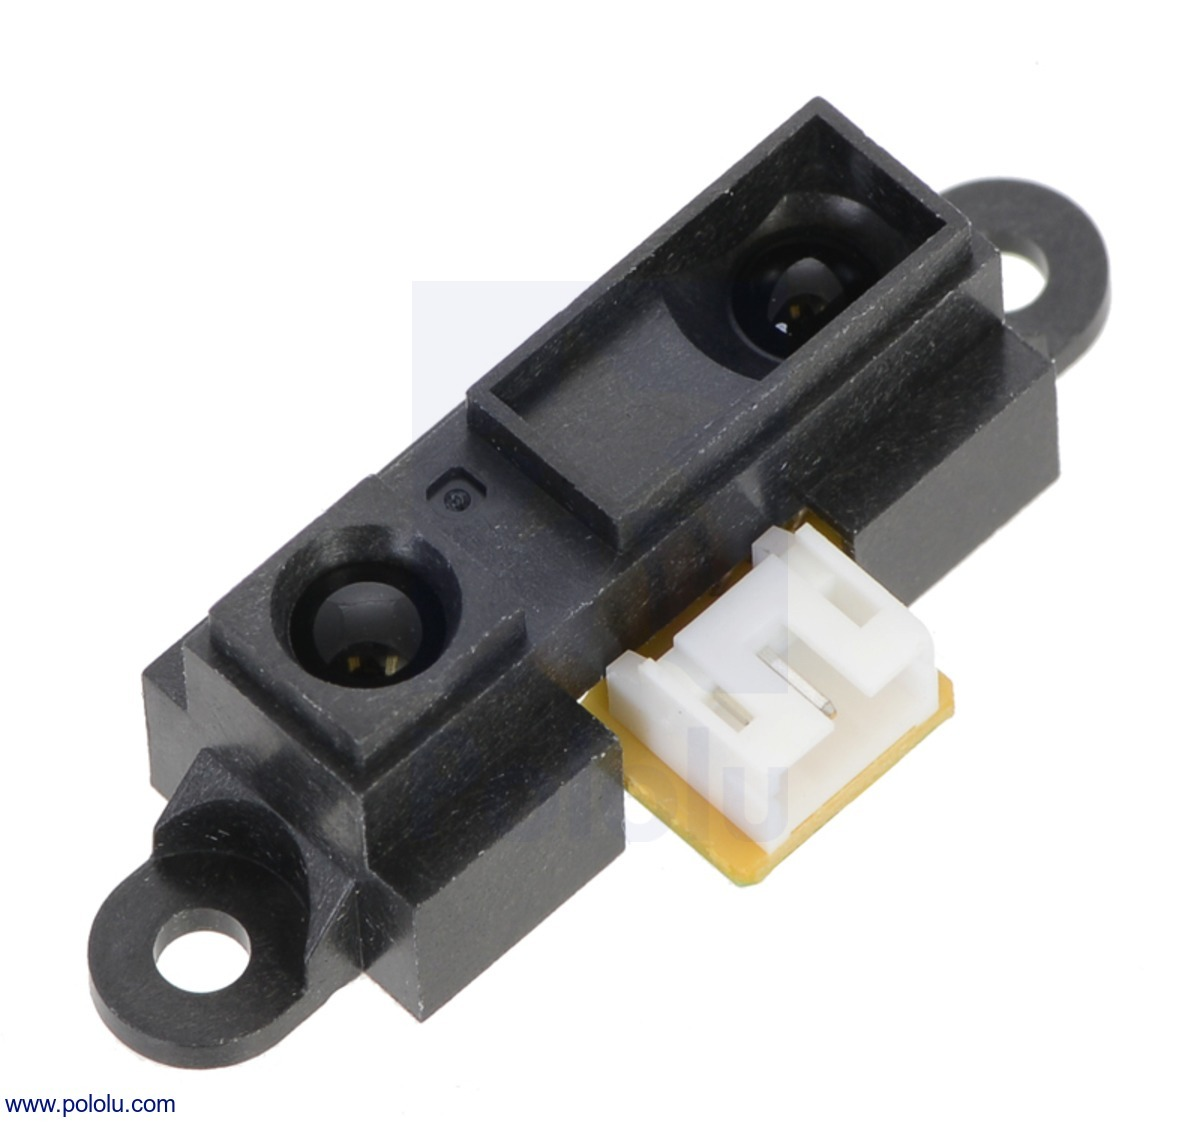
\includegraphics[height = 100]{Capteurs_d.jpg}
    \caption{Capteur de distance : \textit{SHARP GP2D120X}\cite{captdist}.}
    \label{fig:captdist}
    \end{minipage}
    \hfill
    \begin{minipage}[c]{.46\linewidth}
    \centering
    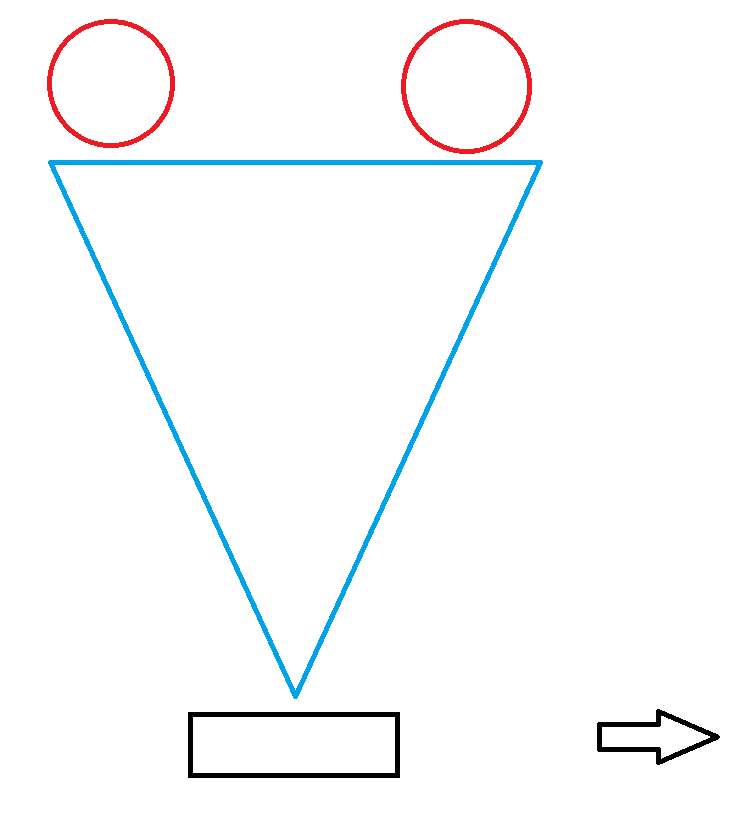
\includegraphics[height = 100]{capteurs_horizontaux.png}
    \caption{cône de détection horizontal}
    \label{fig:cônedetect}
    \end{minipage}
\end{figure}


\subsection{Agencement des composantes et conception}

\begin{figure}[H]
    \begin{minipage}[c]{.46\linewidth}
        \centering
        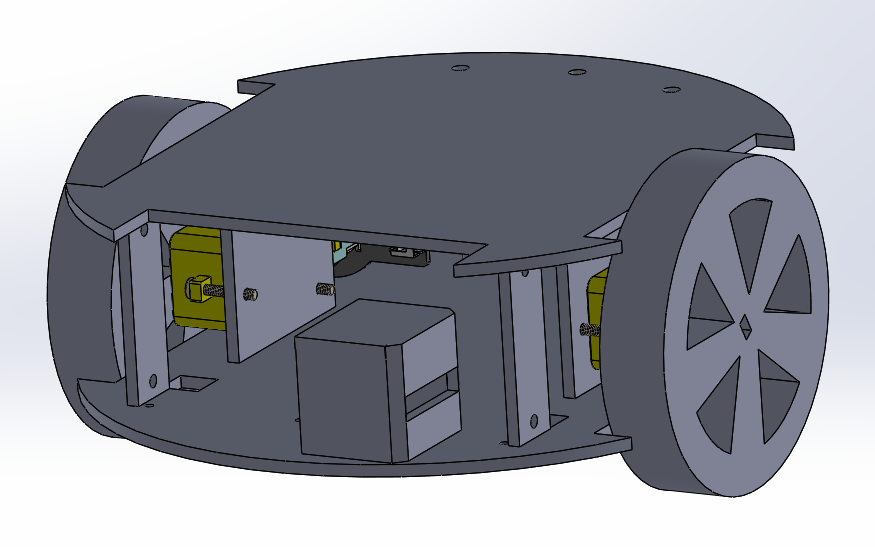
\includegraphics[scale = 0.3]{Chassis_av_cote.png}
        \captionof{figure}{\label{fig:chasavt}Avant du châssis sans composantes vu en plongée}
    \end{minipage}
    \hfill
    \begin{minipage}[c]{.46\linewidth}
        \centering
        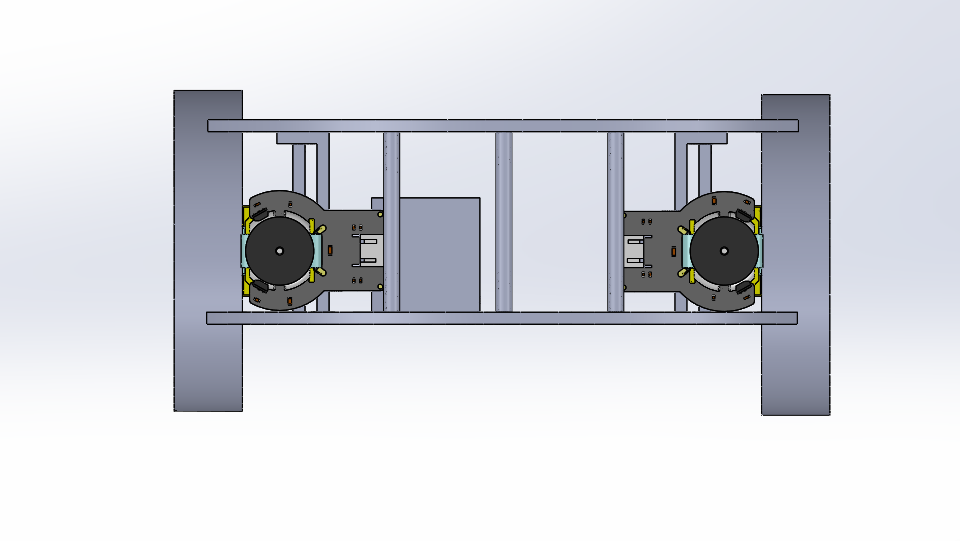
\includegraphics[scale = 0.3]{Chassis_arr.png}
        \captionof{figure}{\label{fig:chasarr}Arrière du châssis sans composantes}
    \end{minipage}
\end{figure}

Le véhicule à proprement parlé est composé d'un châssis circulaire pour se mouvoir avec plus de facilité en prenant le moins de place possible. Ce dernier se sépare en deux étages différents permettant un espace plus important pour les composants et un meilleur équilibre car son centre de gravité est plus bas et la masse est mieux répartie. Cela permet également de réduire la taille du véhicule, la hauteur étant privilégiée à l'augmentation du diamètre afin d'éviter de taper dans les tubes en se déplaçant. Deux encoches sont prévues pour y insérer les roues. Un autre avantage de cette division en deux étages vient du fait que les câbles d'alimentation et ceux servant à la transmission d'informations entre les composants passeront entre les deux plaques et seront donc cachés sans risque de frottement quelconque avec les roues ou avec l'environnement extérieur. Les moteurs se situent entre les deux plaques comme montré sur les figures \ref{fig:chasavt} \& \ref{fig:chasarr} ci-dessus. Les deux plaques sont fixées entre elles par un ensemble de tubes filetés à l'arrière permettant de visser les deux plaques. A l'avant, la plaque du haut est soutenue par des plaques verticales visibles sur la figure \ref{fig:chasavt}. Ainsi, le châssis du véhicule tient solidement ensemble et il n'y aura aucun jeu pendant le mouvement du robot. Les moteurs sont vissés sur les plaques verticales placées au centre du véhicule entre les deux plaques et les roues sont attachées aux moteurs.
\newline

\begin{figure}[H]
    \begin{minipage}[c]{.46\linewidth}
        \centering
        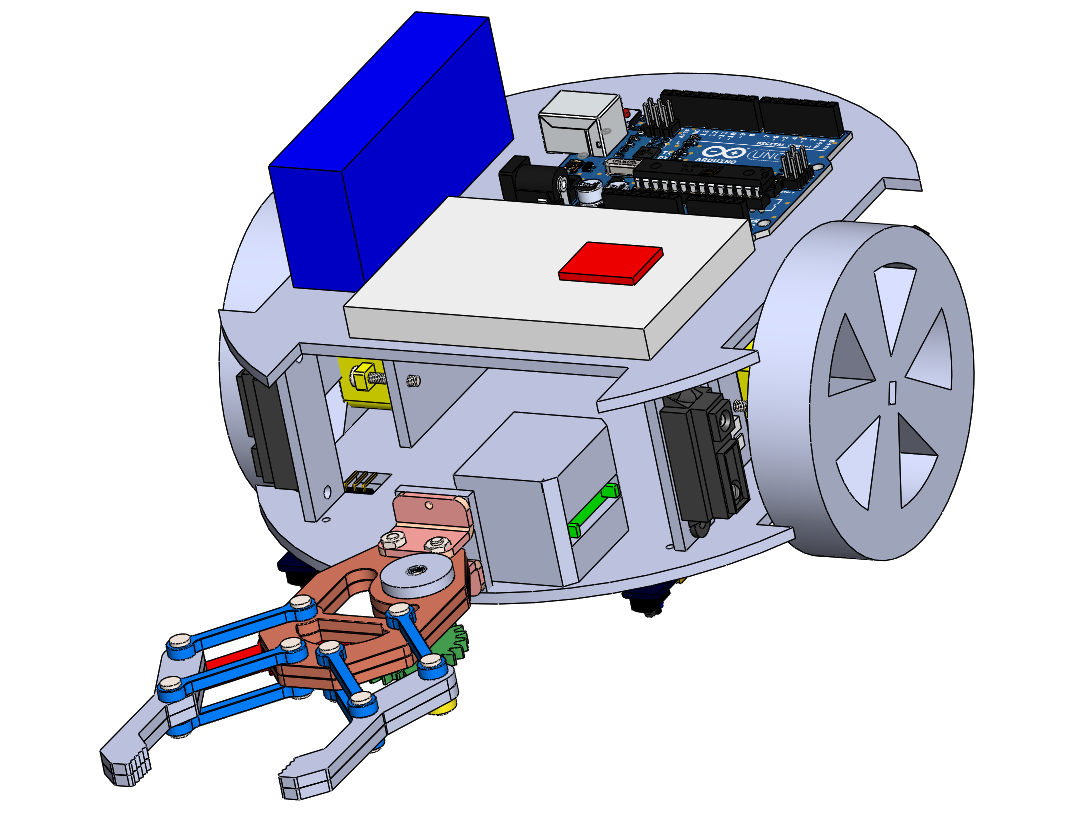
\includegraphics[scale = 0.3]{veh_av_cote.png}
        \captionof{figure}{\label{fig:vehavt}Avant du véhicule vu en plongée avec la pince baissée.}
    \end{minipage}
    \hfill
    \begin{minipage}[c]{.46\linewidth}
        \centering
        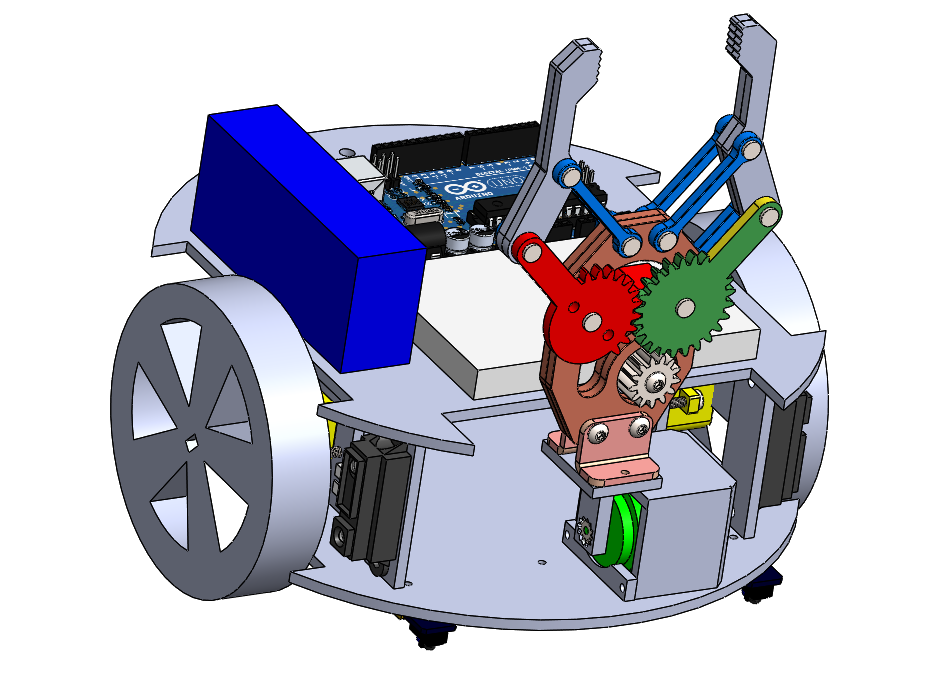
\includegraphics[scale = 0.3]{veh_av_cote_ph.png}
        \captionof{figure}{\label{fig:vehavtph}Avant du véhicule avec la pince levée.} 
    \end{minipage}
\end{figure}

Les composantes principales, à savoir l'Arduino Uno, la batterie (en bleu sur l'image) et le breadboard (en gris clair) sur lequel est positionné le contrôleur de moteur (en rouge), sont placés sur la plaque supérieure. Les capteurs sont mis en dessous et sur les côtés du châssis comme montré sur les images. Les composantes principales seront fixés à l'aide de velcro afin de pouvoir changer leur position aisément si nécessaire. Les capteurs, quant à eux, seront vissés sur les plaques via des supports prévus à cet effet. La pince est positionnée à l'avant du véhicule et le châssis supérieur est creusé pour permettre à la pince de s'élever à 90 degrés. La pince est fixée via un moteur vissé entre les étages et permettant de la faire monter. Ce dernier est modélisé en vert sur les figures \ref{fig:vehavt} et \ref{fig:vehavtph}. Le moteur de la pince est fixé dans le support visible à l'avant du véhicule. Le moteur fermant la pince est attaché à cette dernière et s'élèvera donc avec elle. Il n'est pas modélisé sur le véhicule pour des raisons de lisibilité.

La conception en tant que telle est effectuée, comme la pince, via le logiciel \textit{SolidWorks}. Les châssis supérieurs et inférieurs sont modélisés et imprimés séparément. Des trous sont positionnés à des emplacements stratégiques pour permettre de fixer les composants à l'endroit nécessaire et de visser les plaques entre elles.


%\subsection{La tortue, le design}

\section{Simulation}

La simulation a eu pour but de tester les stratégies possibles et de les comparer afin de choisir la plus adaptée à la problématique. Pour cela, il a fallu modéliser le véhicule à échelle, son déplacement et les contraintes inhérentes à tout déplacement dans la réalité (accélération au démarrage, inertie,...). Cette simulation a été effectuée sur \textit{Python} via le module \textit{Pygame} \cite{pyginf}. Il s'agit d'un module graphique open source souvent utilisé pour le jeu vidéo \cite{pygjeu}  dû à sa puissance et sa richesse mais qui est donc parfaitement adapté à la simulation.
\newline

\begin{figure}[H]
    \centering
    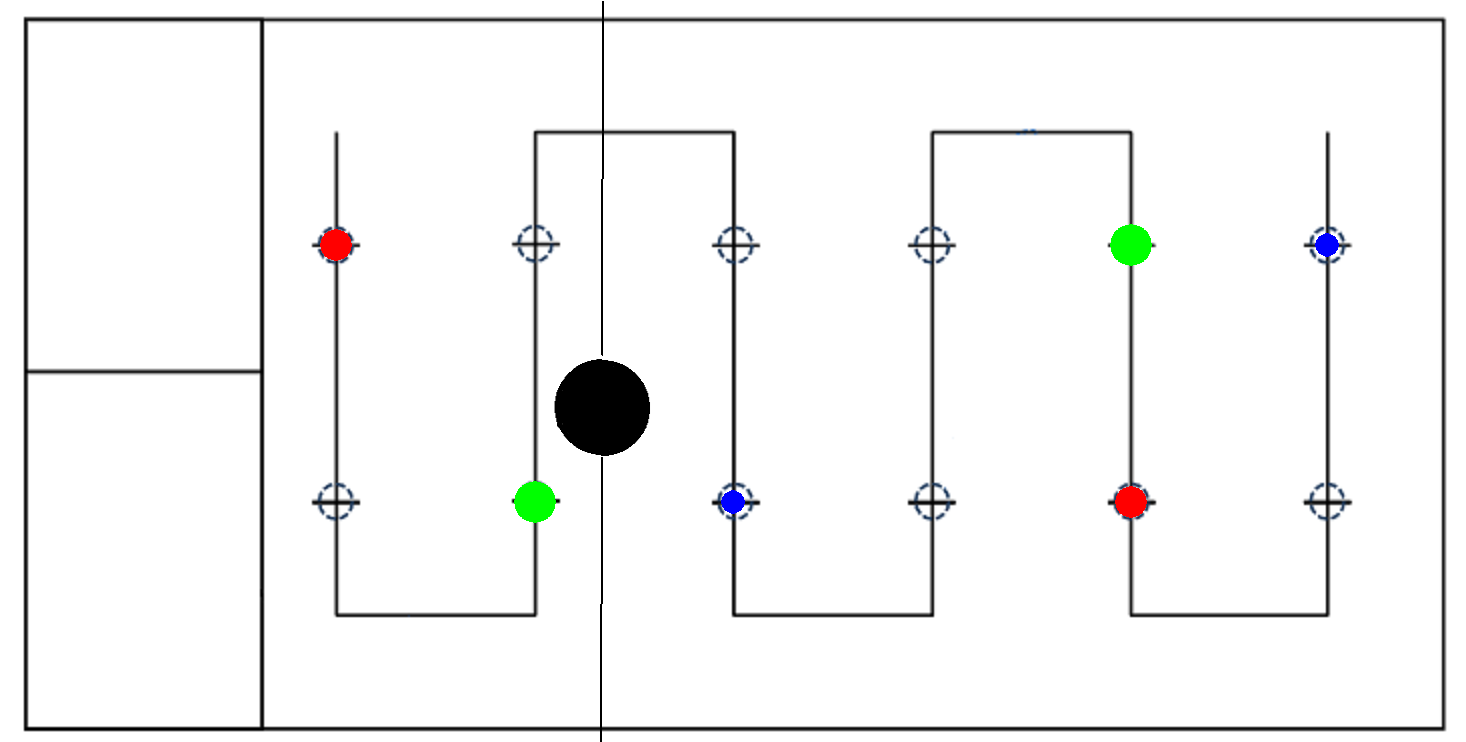
\includegraphics[scale = 0.2]{simu_cyl.png}
    \captionof{figure}{Simulation du véhicule se mouvant sur le terrain.}
    \label{vehmouv}
\end{figure}

 La simulation en elle-même consiste en une fenêtre reproduisant le terrain sur lequel le véhicule se déplacera comme illustré par exemple sur la figure \ref{vehmouv}. Il suffit ensuite de créer l'objet "véhicule" sur ce terrain qui se déplace et interagit avec son environnement. Ce véhicule est modélisé par une boule noire. Les lignes sur les côtés du véhicule représentent les capteurs situés de part et d'autre du véhicule pour la détection des tubes. Les boules bleues, rouges et vertes correspondent respectivement aux tubes de petit, moyen et grand diamètre.\\
 
 Comme expliqué précédemment, Une loi inertielle a été simulée dans le code pour rendre la simulation plus proche de la réalité. En effet, dans la réalité, un véhicule ne démarre pas à 40$km/h$ mais passe d'abord par une phase d'accélération. Dans le code, cela a été imité en obligeant le véhicule à accélérer petit à petit. Ce principe inertiel a été évidemment aussi appliqué à la décélération. Une vitesse maximale a été fixée à $0.5m/s$ car notre véhicule sera également limité à une vitesse de cet ordre. De même, une accélération maximale a été imposée à $1.25m/s^2$
 
 \begin{figure}[H]
    \begin{minipage}[c]{.46\linewidth}
        \centering
        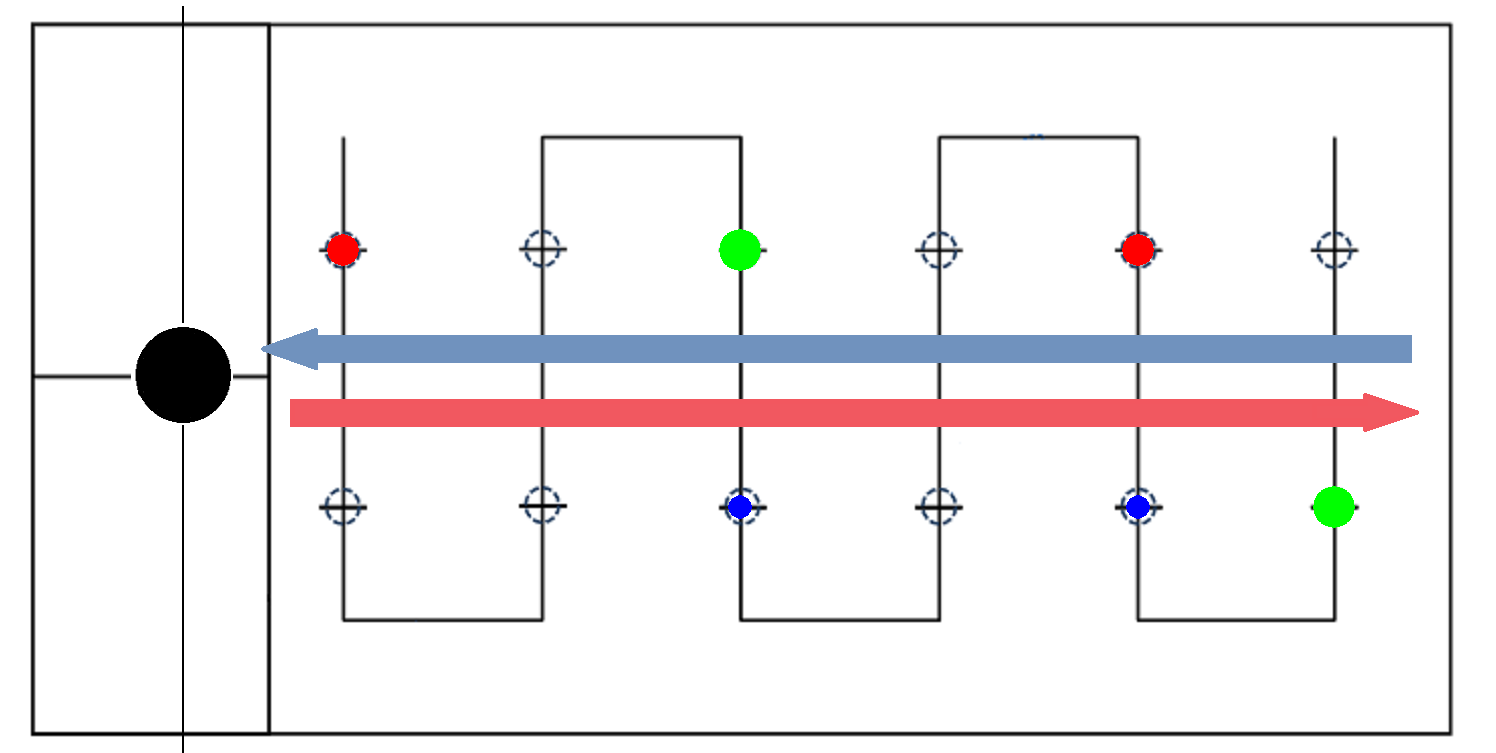
\includegraphics[scale = 0.15]{simu_veh.png}
        \caption{Phase 1 : détection}
    \end{minipage}
    \hfill
    \begin{minipage}[c]{.46\linewidth}
        \centering
        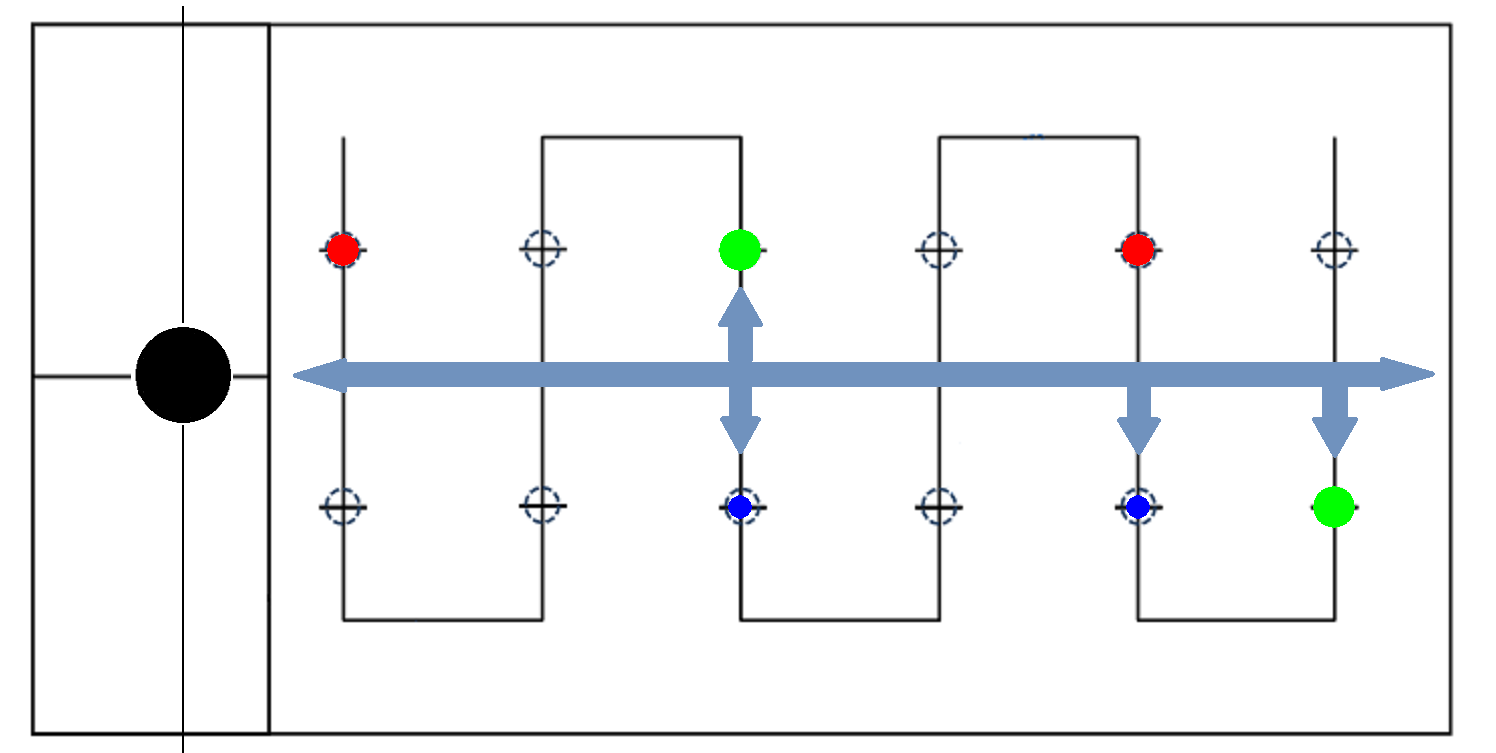
\includegraphics[scale = 0.15]{simu_veh2.png}
        \caption{Phase 2 : transport}
    \end{minipage}
 \end{figure}
 
L'accomplissement de la tâche du véhicule se divise en plusieurs phases. La première consiste en une phase de détection durant laquelle le véhicule va en ligne droite en ralentissant lorsqu'il détecte les tapes noires afin d'avoir des mesures plus précises. Le véhicule retourne ensuite à son point de départ en ayant en mémoire les emplacements des tubes à prendre et leur diamètres respectifs. La seconde phase se découpe en quatre étapes durant lesquelles le robot va prendre les petits et grands tubes et les ramener dans les zones prévues.
 
Comme expliqué précédemment, la méthode de mesure choisie consiste à mesurer le tube à distance en mesurant le temps durant lequel le capteur détecte le tube et en en déduisant son diamètre connaissant la vitesse du véhicule. Pour éliminer les erreurs de détection au maximum, il faut créer des intervalles de mesure correspondant aux trois diamètres différents. Une fois ces intervalles créés, la vitesse du véhicule étant toujours la même lors de sa phase de détection, il n'y a théoriquement plus aucune erreur. Cette méthode s'est donc avérée parfaitement efficace dans les simulations. 
 

\section{Fonctionnement du système}

L'\textit{Arduino Uno} doit être capable de gérer les différentes taches telles que le déplacement (commande moteur), la détection via les différents capteurs (aussi bien les mesures et reconnaissance des tubes que la détection des lignes noires pour corriger la position), ainsi que le contrôle de la pince et de son système élévateur.

Premièrement, une consigne de déplacement sera envoyée aux moteurs des roues par l'Arduino, en l'occurrence une accélération comme point de départ. Ensuite, l'encodeur optique du moteur renverra une information à l'Arduino, faisant entrer par après l'odométrie et la régulation en jeu, détaillées dans la Section \ref{sec:odo} "Odométrie et Régulation" page \pageref{sec:odo}. Celles-ci permettent respectivement au véhicule de connaître sa position sur le plateau et de maintenir la consigne reçue malgré les imperfections de l'environnement, des composants, etc. Une fois le véhicule mis en route, la phase de détection débute.

Tout d'abord les deux capteurs de bords renvoient une information donnant à l'\textit{Arduino} une indication sur les différentes lignes noires rencontrées. Cela permet au contrôleur de corriger la trajectoire du véhicule en envoyant une nouvelle consigne moteur en cas de déportation de sa trajectoire prévue, comme expliqué au point \ref{subsec:capteurs}. La deuxième partie de la détection concerne la reconnaissance des différents tubes. Les capteurs infrarouges renvoient une information en tics à l'Arduino lorsque leur faisceau est coupé par un tube. Les tics correspondent au nombre de fois que la fonction principale est appelée par seconde, il suffit ensuite de transformer les tics en secondes pour pouvoir déterminer le diamètre du tube détecté. Un petit tube renverra un plus petit nombre de tics qu'un grand car le temps pour le dépasser est plus petit, comme expliqué précédemment.

La dernière tâche de l'Arduino est le contrôle de la pince. Il y a deux étapes différentes, pouvant être potentiellement combinées. Il faut tout d'abord envoyer la consigne au $1^{er}$ moteur pour que la pince se ferme. Ensuite, il faut ordonner au second moteur de relever la pince. Il est envisageable d'envoyer une seule consigne qui imposerait de fermer et de relever la pince en même temps. Cela aurait l'avantage d'alléger la tâche de l'Arduino et d'accélérer le processus.\\

Un autre point à considérer est l'alimentation des différents composants. Tout d'abord, une batterie Lipo alimente l'Arduino. Les moteurs seront eux alimentés par un boîtier à piles. Ce dernier choix n'est pas entièrement défini, le type ainsi que le nombre de piles restant encore à déterminer. 


\section{\label{sec:odo}Odométrie et Régulation}

\subsection{Le système d'odométrie}

Comme expliqué à la section \ref{sec:choix}, la stratégie mise en place par l'équipe ne se base en aucun cas sur un suivi de ligne par le robot, que ce soit pour la phase de détection ou pour celle de déplacement des flacons. De ce fait, le prototype ne peut se servir de ces lignes comme repère de position sur le terrain. C'est pourquoi il a fallu développer un système permettant au robot de se repérer dans son environnement, et ce tout au long de la tâche qu'il exécute. C'est ici qu'intervient l'odométrie.

L'odométrie est un module ingénieux à implémenter au robot pour que celui-ci soit en mesure d'avoir accès à sa position approximative ainsi qu'à son orientation à l'instant même où il en a besoin. Il est important de préciser qu'une odométrie cartésienne à deux dimensions selon les axes x et y suffit dans notre cas étant donné que l'environnement dans lequel évolue le véhicule est une surface plane à l'horizontale.\\

La mise en pratique d'un tel système nécessite quelques composantes indispensables. Effectivement, il s'agit de se munir de capteurs appelés encodeurs optiques qui mesurent le nombre de tours effectués par les arbres moteurs, sous forme de tics, durant un intervalle de temps défini, ce qui permet d'avoir accès au déplacement du robot, tout ceci étant traité par l'Arduino jouant le rôle de centre d'opérations et de calculs. Ces calculs de position et d'orientation du robot peuvent être réalisés à partir de deux méthodes différentes.\\
\textbf{Approximation par segment de droite:} la trajectoire du robot peut est découpée en déplacements infinitésimaux rectilignes suivant l'orientation précédente. (voire Figure \ref{fig:approx})\\
\textbf{Approximation par arc de cercle:} la trajectoire du robot est décomposée en arcs de cercle infinitésimaux.\\

Étant donné que ces deux techniques se retrouvent être équivalentes si les mesures se font à fréquence assez élevée, la première méthode est choisie étant donné qu'elle nécessite des calculs moins lourde.\cite{noauthor_robotics:odometrie_2014} Le raisonnement résumant celle-ci est développé ci-dessous et schématisé sur la figure \ref{fig:approx}.\\

A l'instant où l'on a besoin de connaître l'état du robot, c'est-à-dire sa position et son orientation, il s'agit tout d'abord de récupérer les informations détenues par les encodeurs. Il est ensuite nécessaire de transformer celles-ci en variation de distance et d'angle. Pour ce faire, il faut avoir préalablement déterminé les coefficients de transformation de distance de chacune des codeuses par méthode expérimentale.\cite{guyot_[tutoriel]_2016} Ainsi, la détermination des coefficients de transformation de distance gauche et droit consiste à observer les informations relevées par les encodeurs lors de déplacements rectilignes.\\
\begin{figure}[H]
    \centering
    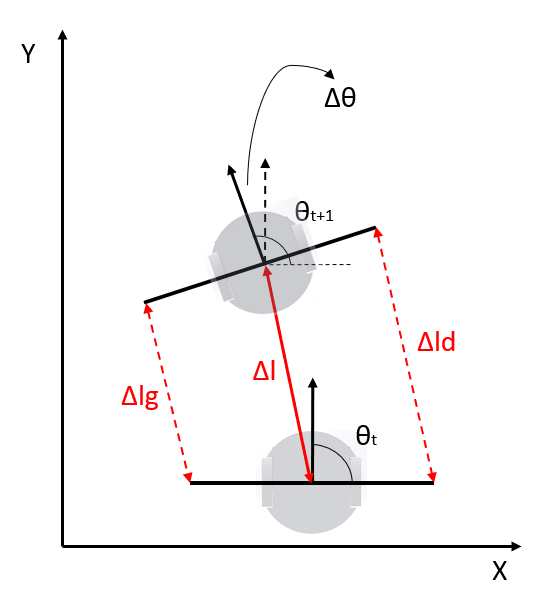
\includegraphics[scale = 1]{approxsegment.PNG}
    \caption{Schématisation de l'approximation par segment de droite}
    \label{fig:approx}
\end{figure}

Sur un intervalle de temps $\Delta$t:\\ \\
Soit le coefficients de transformation de distance $coeff_{D}$\\ 
Soit les informations des encodeurs $x_{tic_{D}}$ et $x_{tic_{G}}$\\
Soit $\Delta l_{D}$ la variation en terme de distance de la roue droite\\
Soit $\Delta l_{G}$ la variation en terme de distance de la roue gauche\\


\begin{equation*}
    \Rightarrow\left\{
      \begin{aligned}
        \Delta l_{D} & = coeff_{D}*x_{tic_{D}}\\
        \Delta l_{G} & = coeff_{G}*x_{tic_{G}}
        \end{aligned}
    \right.
\end{equation*}\\\\\\
Dès lors, les déplacements respectifs des roues donnent accès au déplacement global du robot ainsi qu'à sa nouvelle orientation :\\\\
Soit $\Delta l_{moy}$ la distance parcourue par le centre du robot\\
Soit $\Delta\theta$ la variation d'orientation du robot\\
Soit L la distance entre les deux roues du robot
\begin{equation*}
    \Rightarrow\left\{
      \begin{aligned}
        \Delta l_{moy}  & =\frac{\Delta l_{D}+\Delta l_{G}}{2}\\
        \Delta\theta  & = \arctan(\frac{\Delta l_{D}-\Delta l_{G}}{L}) \approx \frac{\Delta l_{D}-\Delta l_{G}}{L}
        \end{aligned}
    \right.
\end{equation*}\\\\
En ce qui concerne le reste du raisonnement, il faut convertir les variations de distance en déplacements selon l'axe x et l'axe y. Le déplacement étant considéré ici comme un segment de droite, il faut prendre en compte la dernière orientation du robot\cite{noauthor_robotics:odometrie_2014}:\\
Soit $\theta_{t-1}$ l'orientation obtenue à la dernière mesure
\begin{equation*}
    \Rightarrow\left\{
      \begin{aligned}
        \Delta x = \Delta l*\cos(\theta_{t-1})\\
        \Delta y = \Delta l*\sin(\theta_{t-1})
        \end{aligned}
    \right.
\end{equation*}\\\\
Pour finir, le calcul de la position et de l'orientation du robot à l'instant présent se fait comme suit:
\begin{equation*}
    \Rightarrow\left\{
      \begin{aligned}
        x_{t} = x_{t-1} + \Delta x\\
        y_{t} = y_{t-1} + \Delta y\\
        \theta_{t} = \theta_{t-1} + \Delta\theta\\
        \end{aligned}
    \right.
\end{equation*}\\\\
Dès lors, le bloc odométrie permet à n'importe quel moment de sortir un triple ($x_{t}$, $y_{t}$, $\theta_{t}$) correspondant à l'état du robot à cet instant précis, c'est-à-dire respectivement sa coordonnée selon x, sa coordonnée selon y et son orientation. Par ailleurs, les approximations faites ci-dessus sont assez grossières et peuvent ainsi induire une dérive considérable sur de longs trajets, c'est pourquoi la fréquence de mesure se doit d'être assez élevée pour rendre les déplacements infinitésimaux pris en compte.

\subsection{La régulation PID}

\subsection{Objectif}

Maintenant que le prototype sait où il se trouve lors de son évolution dans son environnement, il est envisageable de le faire se déplacer d'un endroit à un autre, afin de réaliser la stratégie mise en place par l'équipe. Pour ce faire, il faut lui donner des consignes de position et d'orientation adaptées qu'il mettra en oeuvre au moment voulu. Le problème est qu'en réalité, le robot va être confronté à des imperfections imprévisibles telles que des frottements secs au sein des moteurs, ou encore des différences de fabrication entre les moteurs censés être similaires. Celles-ci fausseront le déplacement réellement effectué par le robot. En d'autres termes, elles lui feront dévier de son objectif quant à la réalisation des consignes ordonnées. C'est pourquoi il est nécessaire de mettre en place un système de régulation permettant au véhicule de prendre en compte les erreurs entre la consigne à effectuer et ce qu'il en est réellement. Ce pour pouvoir minimiser cette erreur, voir potentiellement l'annuler, en rectifiant le comportement du robot au cours du temps. La régulation PID, pour proportionnelle, intégrale et dérivée, est l'une des méthodes les plus utilisées au sein des processus industriels.\cite{le_lann_pid_2007} Elle permet, comme expliqué ci-dessus, d'atteindre et de maintenir un paramètre quelconque aussi près que possible de la consigne demandée, le tout en boucle fermée comme le montre la Figure \ref{fig:boucle}. Pour ce faire, elle modifie l'erreur réelle sur la consigne, calculée à intervalles réguliers à l'aide de capteurs adapté, de manière à obtenir un système asservi ayant le comportement souhaité. Cette modification se fait en faisant intervenir dans les asservissements proportionnel, intégral et dérivée, respectivement, l'erreur de base, la somme totale des erreurs ainsi que la différences des deux dernières erreurs. L'effet que ces différents termes ont sur le système global sera détaillé dans la sous-section \ref{subsec:influence}.\\

\begin{figure}[H]
    \centering
    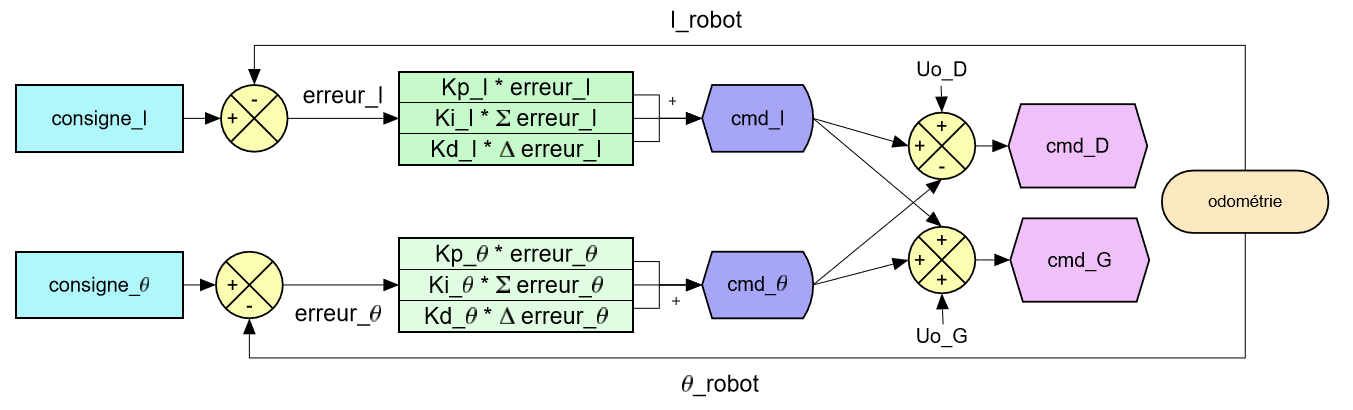
\includegraphics[scale = 0.55]{Capture.PNG}
    \caption{Boucle d'asservissement de position}
    \label{fig:boucle}
\end{figure}\\\\

\subsection{Régulation de position}

Le but étant de déplacer le robot d'un endroit à un autre de la manière la plus précise possible, la régulation se fait donc sur la position du robot. La consigne que le robot reçoit est un couple de coordonnées cartésiennes correspondant à l'endroit où il doit se rendre sur la carte. Cette consigne principale est ensuite décomposée en deux sous-consignes, une consigne de distance $l_{consigne}$ et une consigne d'angle $\theta_{consigne}$, par calculs faisant intervenir des notions vectorielles et trigonométriques.

Tout d'abord il faut savoir que le raisonnement suivant est fait selon un système de coordonnées cartésiennes dont les axes x et y suivent respectivement la largeur et la longueur de la carte et une orientation suivant le système trigonométrique. La distance à parcourir par le robot s'obtient en calculant la norme du vecteur construit par ses deux points extrêmes. Le calcul de l'angle à effectuer par le robot pour se trouver en face de sa cible utilise la fonction atan2(y,x) qui est une fonction à 2 variables permettant en pratique de trouver l'angle construit par la droite passant par l'origine (0,0) et le point (x,y) et l'axe des x positifs.\cite{cochelin_positionnement_nodate}\\\\
\begin{figure}[H]
    \centering
    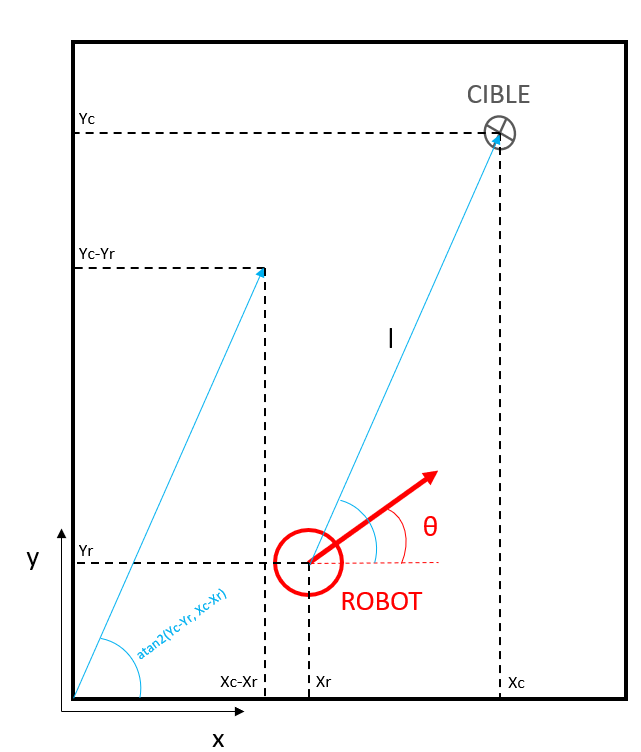
\includegraphics[scale = 1]{atan2.PNG}
    \caption{Représentation graphique du calcul des consignes}
    \label{fig:atan}
\end{figure}\\


A l'instant t où le robot reçoit une consigne:\\\\
Soit la position cible ($x_{cible}$, $y_{cible}$)\\
Soit l'état du robot à cet instant (x, y , $\theta$)
\begin{equation*}
    \Rightarrow\left\{
        \begin{aligned}
            l_{consigne} & = \sqrt{(x_{cible}-x)^2+(y_{cible}-y)^2}\\ 
            \theta_{consigne_{rad}} & = atan2(y_{cible}-y, x_{cible}-x)-\theta
        \end{aligned}
    \right.
\end{equation*}\\
Avec $\theta_{consigne_{rad}}$ compris entre -$\pi$ et $\pi$ radian\\\\
\begin{equation*}
    \Rightarrow\left\{
        \begin{aligned}
            \theta_{consigne_{deg}} = l_{consigne_{rad}}*\frac{180}{\pi}
        \end{aligned}
    \right.
\end{equation*}\\
Avec $\theta_{consigne_{deg}}$ maintenant compris entre -180$\degree$ et 180$\degree$\\\\
Il s'agit ensuite de calculer l'erreur selon la consigne de distance ($erreur_{l}$) ainsi que celle selon la consigne d'angle ($erreur_{\theta}$) afin d'utiliser celles-ci dans le bloc d'asservissement. Pour ce faire, il faut récupérer le triple (x, y, $\theta$) à la fréquence d'échantillonnage afin d'avoir une erreur qui évolue avec l'état du robot.\\\\
Soit (x, y, $\theta$) l'état du robot à l'instant où il a reçu la consigne.\\
Soit (x(t), y(t),$\theta$(t)) l'état du robot à l'instant où l'erreur doit être calculée\\
Soit $l_{consigne}$ l'$erreur_{l}$ initiale\\
Soit $\theta_{consigne}$ l'$erreur_{\theta}$ initiale

\begin{equation*}
    \left\{
        \begin{aligned}
            erreur_{l} & = l_{consigne} - \sqrt{(x(t)-x)^2+(y(t)-y)^2}\\
            \Sigma_{erreur_{l}} +&= erreur_{l}\\
            \Delta_{erreur_{l}} & = erreur_{l} - erreur_{l_{old}}\\
            erreur_{l_{old}} & = erreur_{l}\\
            \end{aligned}
    \right.
\end{equation*}
\begin{equation*}
    \Rightarrow commande_{l} =  Kp_{l}*erreur_{l}+Ki_{l}*\Sigma_{erreur_{l}}+Kd_{l}*\Delta_{erreur_{l}}
\end{equation*}

\begin{equation*}
    \left\{
        \begin{aligned}
            erreur_{\theta} & = \theta_{consigne} - \theta(t)\\
            \Sigma_{erreur_{\theta}} +&= erreur_{\theta}\\
            \Delta_{erreur_{\theta}} & = erreur_{\theta} - erreur_{\theta_{old}}\\
            erreur_{\theta_{old}} & = erreur_{\theta}\\
        \end{aligned}
    \right.
\end{equation*}

\begin{equation*}
    \Rightarrow commande_{\theta} = Kp_{\theta}*erreur_{\theta}+Ki_{\theta}*\Sigma_{erreur_{\theta}}+Kd_{\theta}*\Delta_{erreur_{\theta}}
\end{equation*}
Le châssis choisi étant fixe, il faut appliquer des vitesses différentielles pour effectuer un changement de direction. C'est pourquoi la commande d'angle doit contribuer positivement pour l'un des moteurs et négativement pour l'autre. On parle d'asservissement différentiel, parfois également appelé asservissement polaire ou en alpha-delta.\cite{rouviere_asservissement_2007}


\begin{equation*}
    \Rightarrow\left\{
        \begin{aligned}
           commande_{moteur_{droit}} & = commande_{l} - commande_{\theta}\\
           commande_{moteur_{gauche}} & = commande_{l} + commande_{\theta}
           \end{aligned}
    \right.
\end{equation*}\\
Pour finir, il faut s'assurer que les tensions finales correspondant aux commandes à envoyer aux moteurs droit et gauche ne dépassent pas les valeurs nominales de ceux-ci. Il faut également rajouter aux commandes finales les tensions minimales respectives $U_{0_{D}}$ et $U_{0_{D}}$ des moteurs, étant donné que c'est à partir de celles-ci que ces derniers commencent réellement à actionner leur essieux. Cela permet ainsi d'obtenir une réactivité optimale de la part du système. Les commandes finales sont donc :
\begin{equation*}
    \Rightarrow\left\{
        \begin{aligned}
           commande_{moteur_{droit}} & = commande_{l} - commande_{\theta}+U_{0_{D}}\\
           commande_{moteur_{gauche}} & = commande_{l} + commande_{\theta}+U_{0_{G}}
           \end{aligned}
    \right.
\end{equation*}\\

La boucle d'asservissement (Figure \ref{fig:boucle}) résume synthétiquement la régulation de position expliquée ci-dessus.\\

\subsection{\label{subsec:influence}Influence des coefficients\cite{le_lann_pid_2007}}

La régulation proportionnelle engendre, comme son nom l'indique, une commande directement proportionnelle à l'erreur commise. Son but est d'amplifier de manière fictive cet écart afin d'en augmenter la correction réelle, rendant ainsi le système plus vif. En d'autre termes, le coefficient de proportionnalité Kp rend l'erreur plus grande que ce qu'elle n'est vraiment, diminuant ainsi le temps de montée en régime du système. C'est la partie la plus intuitive de la régulation de position : plus le robot est loin de sa cible, plus la puissance délivrée aux moteurs est élevée. De la même manière, plus le robot se rapproche de sa cible, plus la puissance délivrée aux moteurs est faible.

Pour ce qui est de la régulation intégrale, elle vient compléter l'erreur statique laissée par la partie proportionnelle. En effet, une fois la consigne presque atteinte, la commande résultante en tension est trop faible pour actionner les moteurs. Dès lors, le terme intégral prend en compte l'accumulation des erreurs mesurées tout au long des corrections établies pour atteindre l'objectif. Par conséquent, contrairement au terme proportionnel, le coefficient intégral Ki garde un effet stable sur la commande, et ce même lorsque l'écart est minime. Il faut donc faire attention à ne pas trop élever la valeur de celui-ci pour éviter les dépassement trop importants de la consigne désirée, ce qui entraînerait des oscillations indésirables autour de la valeur cible.

Le terme dérivé influence quant à lui la commande finale en tenant compte de la différence entre les deux dernières erreurs successives. Cela signifie en pratique qu'il permet d'anticiper quand sera atteinte la consigne en considérant la vitesse à laquelle évolue l'erreur. Effectivement, plus le robot s'approche rapidement de la cible, moins la commande liée au terme dérivé délivre de la puissance - et inversement. Il paraît dès lors logique que cet élément de régulation s'oppose directement à l'effet du coefficient de proportionnalité. Son rôle est majeur lorsque le robot est sur le point d'atteindre sa cible car, tandis que le terme proportionnel est presque nul et que le terme intégral continue d'actionner le système, le coefficient dérivé permet de freiner le robot, diminuant ainsi les oscillations ainsi que le temps de stabilisation de celui-ci.\\

\subsection{Détermination des coefficients\cite{le_lann_pid_2007}}

Maintenant que l'influence de chacun des coefficients intervenant dans le bloc d'asservissement est connu, il s'agit de déterminer leurs valeurs de manière à obtenir un système le plus stable, précis et rapide possible. La technique la plus fine pour ce faire serait de modéliser l'entièreté du système, ce qui n'est pas réalisable à l'échelle du projet étant donné que certains paramètres ne sont pas accessibles. Effectivement, que ce soient les défauts de fabrications, les frottements secs ou encore le jeu au sein des moteurs, aucun de ces paramètres ne peut être parfaitement pris en compte, ce qui rend l'étude mathématique du système impossible. De ce fait, la démarche à mettre en oeuvre doit être empirique, c'est-à-dire qu'elle doit être basée sur des tests dits d'essais-erreurs.

Pour effectuer des recherches dans le vide, l'équipe s'est appuyée sur la méthode empirique de Ziegler-Nichols.\\ 
Pour la mettre en pratique, il faut dans un premier temps mettre les termes intégral et dérivé à zéro, puis augmenter le gain proportionnel jusqu'à atteindre des oscillations stables autour de la consigne. Les deux autres coefficients se détermine alors comme suit:\\\\
Soit $Kp_{limite}$ le coefficient proportionnel engendrant les oscillations.\\
Soit $T_{oscillation}$ la période des oscillations obtenues.

\begin{equation*}
    \Rightarrow\left\{
        \begin{aligned}
            Kp & = 0.6*Kp_{limite}\\
            Ki & = \frac{1}{0.5*T_{oscillation}}\\
            Kd & = 0.125*T_{oscillation}
           \end{aligned}
    \right.
\end{equation*}

Une fois ces coefficients pré-déterminés, il est question de faire varier légèrement ces derniers de manière à accentuer les effets recherchés, pour finalement approcher le comportement du système le plus adéquat. Généralement, en ce qui concerne la régulation de position, le robot se veut le plus précis possible, c'est-à-dire que l'erreur statique se veut minimale.
\newline

\subsection{Consigne évolutive}

Un problème persiste, malgré le fait que désormais, le comportement du système peut être adapté aux besoins du projet en modifiant les coefficients proportionnel, intégral et dérivée en se basant sur les effets qu'ils engendrent - en plus d'avoir une connaissance suffisante de l'objectif et du fonctionnement de la régulation PID en terme de position. En effet, en demandant au robot de se rendre à un point cible de son environnement, seul le résultat final est régulé par la boucle d'asservissement (voir figure \ref{fig:boucle}), mais en aucun cas la trajectoire du robot n'est considérée. Cela devient problématique en ce sens qu'au delà d'une certaine distance à parcourir, celle-ci étant assez réduite, le robot fait tourner ses moteurs à plein régime sans adaptation aucune de sa vitesse, ce qui mène à une perte de contrôle inévitable. De plus, cela pourrait endommager nos moteurs.

Pour pallier à ce problème, il faut d'implémenter au robot une consigne qui évolue au cours du temps et qui engendre une vitesse de déplacement bien précise chez le robot. Ainsi, la consigne demandée permet de contrôler l'évolution du mouvement effectué par le véhicule pour aboutir au résultat voulu. En ce qui concerne ce mouvement au cours du temps, l'objectif est d'obtenir un prototype se déplaçant - dans la mesure du possible - avec un profil de vitesse trapézoïdal représenté sur la Figure \ref{fig:trapèze}. En d'autres termes, il s'agit de contraindre la puissance délivrée aux moteurs afin que n'importe quelle course ordonnée par une consigne position passe par 3 phases successives bien déterminées : une phase d'accélération constante, suivie d'une phase à vitesse constante, elle-même suivie d'une phase de décélération constante. Le développement suivant reprend le raisonnement permettant d'atteindre une telle ligne de conduite.\\
\begin{figure}[H]
    \centering
    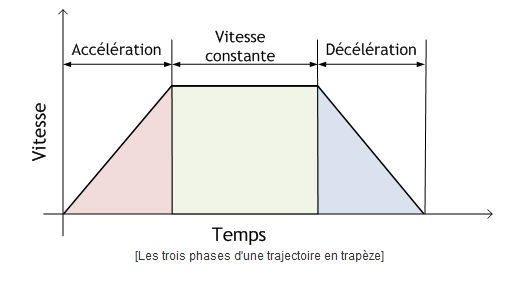
\includegraphics[scale = 1]{Profile_trapeze.png}
    \caption{Profile de vitesse trapézoïdal\cite{noauthor_construction_nodate}}
    \label{fig:trapèze}
\end{figure}

Le calcul du temps $\tau$ que met le robot pour atteindre sa vitesse de croisière se fait simplement comme suit:
\newline

\noindent Soit A l'accélération pour la phase d'accélération constante.\\
Soit $A_{max}$ l'accélération maximale du robot.\\
Soit V la vitesse de croisière pour la phase à vitesse constante.\\
Soit $V_{max}$ la vitesse maximale du robot.
\begin{equation*}
    \left\{
        \begin{aligned}
            A & = \frac{V}{\tau} \Rightarrow \tau = \frac{V}{A}  & (1)\\ 
           \end{aligned}
    \right.
\end{equation*}
La distance parcourue par le robot sur cette phase d'accélération, étant également la distance parcourue lors de la phase de décélération, l'aire sous la pente positive du trapèze c'est-à-dire la zone triangulaire rouge sur la figure \ref{fig:trapèze}.

\begin{equation*}
    \Rightarrow\left\{
        \begin{aligned}
        l_{\tau} & = \frac{A}{2}*\tau^2\\
           \end{aligned}
    \right.
\end{equation*}\\
En substituant $\tau$ par son expression trouvée en (1), on obtient:
\begin{equation*}
    \Rightarrow\left\{
        \begin{aligned}
        l_{\tau} = \frac{V^2}{2A}\\
           \end{aligned}
    \right.
\end{equation*}\\
À ce stade du raisonnement, il faut prendre en considération deux cas particuliers face auxquels peut se retrouver le robot lorsqu'une consigne lui est imposée. En effet, si la consigne de distance est plus petite que la distance parcourue le temps de la phase d'accélération, il paraît évident que le robot ne pourra atteindre sa vitesse de croisière. Dans ce cas, le profil de vitesse devient un profil triangulaire parfois dit profil "bang-bang".\cite{chemori_generation_nodate}\\\\

\underline{Si $consigne_{l}$ $\leq$ l_{$\tau$}}:\\\\
Le fait que la distance parcourue lors de la phase d'accélération est la même que celle parcourue lors de la phase de décélération donne accès au temps $\tau_{bang}$ durant lequel le robot doit accélérer:
\begin{equation*}
    \Rightarrow\left\{
        \begin{aligned}
        \frac{consigne_{l}}{2} = \frac{A*\tau_{bang}^2}{2} \Leftrightarrow \tau_{bang} = \sqrt{\frac{consigne_{l}}{A}}\\
           \end{aligned}
    \right.
\end{equation*}\\
Le mouvement sur la distance aura donc un temps de réalisation global T = 2*$\tau_{bang}$ = $2\sqrt{\frac{consigne_{l}}{A}}$. La fonction continue qui fournit la $consigne_{l_{evo}}$ à transmettre au robot pour générer chez lui un profil de vitesse triangulaire se construit comme suit:
\begin{equation*}
    \left\{
        \begin{aligned}
        l_{evo}(t) & = \frac{A}{2}*t^2 &si : t<\tau_{bang}\\
        l_{evo}(t) & = \frac{A}{2}*(t-\tau_{bang})^2 + l_{\tau_{bang}} &si : t>\tau_{bang}
        \end{aligned}
    \right.
\end{equation*}\\

\underline{Si $consigne_{l}$ $>$ $l_{\tau}$}:\\\\
La distance $l_{\tau}$ parcourue le temps d'atteindre la vitesse de croisière ayant déjà été calculée, il ne reste plus qu'à mesurer la distance à parcourir durant la phase à vitesse constante pour pouvoir accéder au temps de croisière ainsi qu'au temps global d'exécution.

\begin{equation*}
    \left\{
        \begin{aligned}
        l_{V_{cste}} &= consigne_{l} - 2l_{\tau}  = l - \frac{v^2}{A}\\
        \Delta_{V_{cste}} &= \frac{l_{v_{cste}}}{V}  = \frac{A*l-v^2}{AV}\\
        \end{aligned}
    \right.
\end{equation*}\\
\begin{equation*}
    \left.
        \begin{aligned}
        \Rightarrow T = 2\tau + \Delta_{v_{cste}}  = 2\tau + \frac{A*l-V^2}{AV}
        \end{aligned}
    \right.
\end{equation*}\\
Dès lors, la fonction continue de la consigne sur la distance en fonction du temps peut être mise en place. Celle-ci générant cette fois un profil trapézoïdal de vitesse chez le prototype.
\begin{equation*}
    \left\{
        \begin{aligned}
        l_{evo}(t) & = \frac{A}{2}*t^2 &si&: 0<t<\tau\\
        l_{evo}(t) & = V*(t-\tau) + l_{\tau} &si&: \tau<t<T-\tau\\
        l_{evo}(t) & = \frac{A}{2}*(t-T)^2 + l_{v_{cste}} + l_{\tau} & si&: T-\tau < t < T
        \end{aligned}
    \right.
\end{equation*}\\
Maintenant que la fonction génératrice des distances est définie, il s'agit de mettre en place la même démarche pour la consigne sur l'angle. Par ailleurs, ces fonctions doivent être évaluées aux moments propices. En pratique, cela se fait à la fréquence d'échantillonnage de l'asservissement. Bien évidemment, il faut toujours avoir une consigne d'avance, c'est-à-dire que la commande ne dit pas au robot où il est mais bien là où il devrait être.
Si f est la fréquence d'échantillonnage à laquelle s'exécute la régulation PID, cela implique que la période échantillonnage équivaut à $\frac{1}{f}$, ce qui correspond à l'intervalle de temps entre deux itérations. Les fonctions de consignes s'évaluent donc suivant ce modèle.\\
\underline{Si i\textsuperscript{ème} itération} :
\begin{equation*}
    \Rightarrow\left\{
        \begin{aligned}
        consigne_{l_{evo}} = l_{evo}(\frac{1}{f}*(i+1))
        \end{aligned}
    \right.
\end{equation*}\\
En dernier lieu, Il est question de s'assurer que la fréquence d'échantillonage garantit le fait de passer par les points caractéristiques du profil de vitesse c'est-à-dire les sommets de la forme géométrique décrite par celui-ci. Pour ce faire, il suffit que $\tau$ et $\Delta_{V_{cste}}$ soient tous deux des multiples entiers de la période d'échantillonnage $\frac{1}{f}$.
Le système global contrôle désormais à la fois le résultat cible ainsi que la trajectoire du mouvement qui permet d'atteindre ce dernier. 



% \section{Construction et modidifications nécessaires et apportées}

% \section{Tests ?}
% Rapidité du robot à accomplir sa tâche, robustesse, efficacité et précision de l'odométrie, du système de détection, de la régulation OK mais dans futur du projet,\tdot


\section{Project management}

Un SWOT est l'auto-évaluation d'un groupe dans le but de l'aider à mettre en évidence les avantages dont il pourrait tirer profit, d'une part, et les faiblesses qu'il pourrait améliorer, de l'autre. Ce mot est en réalité l'acronyme de \textit{Strengths, Weaknesses, Opportunities, Threats}. Voici le SWOT fait au sein de notre groupe:
\begin{figure}[H]
    \centering
    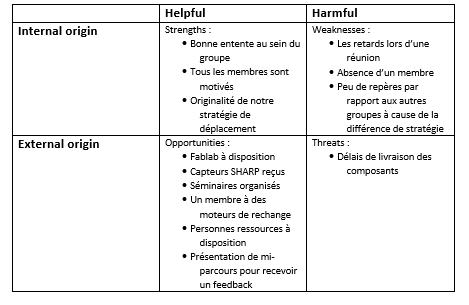
\includegraphics[scale = 1]{swot.png}
    \caption{\label{fig:SWOT}SWOT}
\end{figure}

Pour s'assurer du bon déroulement du projet et de son avancement, notre groupe s'est réuni chaque semaine dans le but de faire un débriefing des dernières avancées et de répartir, le plus équitablement possible, de nouvelles tâches au sein du groupe. La meilleur façon d'avancer rapidement est d'attribuer, à chaque membre du groupe, une tâche bien précise pour s'assurer qu'elle ait bien été effectuée avant la prochaine réunion. En effet, si le groupe n'a qu'une seule tâche globale à effectuer, tout le monde espérera qu'un autre membre la fasse sans que personne ne s'en occupe au final. 
Lors d'une réunion, un membre joue le rôle d'animateur pendant qu'un autre, le secrétaire, s'occupe de noter les points principaux. L'animateur prépare et partage l'ordre du jour de la prochaine réunion, au moins un jour avant celle-ci. Le secrétaire est chargé d'en rédiger le procès verbal et de le publier dans les jours qui suivent.
Ceci est contrôlé de loin par un superviseur dont le rôle est de veiller au bon déroulement du projet tout en restant passif, c'est-à-dire qu'il ne peut pas aider le groupe quant à la réalisation même du prototype. De plus, des échéances doivent être respectées. Divers rapports et présentations orales sont à réaliser pour des dates précises. Afin d'améliorer le partage du travail effectué, tous les fichiers sont mis en ligne sur un dossier Dropbox commun, Slack est employé pour la communication spécifique à un aspect du projet (modélisation, code, etc.), la discussion générale se déroule sur Facebook Messenger, et les rapports de projet sont rédigés sur un document LaTeX coopératif sur Overleaf.



\section{Futur du projet}
% Q2 Ce que l'on pourrait améliorer, à quoi pourrait servir le projet, comment le développer différemment, \tdot
Dès le début du second quadrimestre, le châssis et la pince du robot auront été imprimés. Le robot pourra être assemblé avec le reste de ses composants.
Les tests en situation réelle pourront donc commencer dans le but de vérifier si les différentes étapes du mode opératoire mis en place fonctionnent, ainsi que les composants, le design, etc. En effet, il va falloir s'assurer que le robot suit bien le trajet désiré tout en différenciant les différents flacons grâce à ses deux capteurs infrarouges, que la pince agrippe suffisamment les flacons pour qu'elle puisse les déplacer jusqu'à leur zone de dépôt. Pour ce faire, une grande phase de programmation est encore à accomplir. Un travail intensif devrait être de mise car cette période de travail sera courte et il est peu probable que le robot fonctionne entièrement du premier coup.

Une fois le robot terminé, il pourra se rendre très utile pour diverses applications industrielles. Il pourra, par exemple, diminuer la main d'oeuvre nécessaire au sein d'une usine de tri et faire gagner un temps précieux aux employés, permettre un rangement automatisé dans des zones difficiles d'accès pour un bras humain, amener un médicament au comptoir d'une pharmacie pour que le pharmacien ne doive interrompre son explication des effets secondaires, etc. Cependant, il pourra, d'ici là, être exposé lors du Printemps des Sciences et intriguera quantité de visiteurs passionnés de robotique.

\section{Conclusion}
Ce projet se révèle très enrichissant dans la mesure où il a consisté en une approche concrète du métier d’ingénieur. En effet, la prise d’initiative, le respect des délais et le travail en équipe seront des aspects essentiels de notre futur métier. De plus, il a permis d’appliquer nos connaissances en robotique à un domaine pratique, qui se révèle aujourd’hui d’intérêt général au vu de l'automatisation du travail.
% \section{Remerciements}
% Pour le matériel reçu, le code partagé, l'aide quelconque, etc \tdot

%\newpage
%\begin{appendices}
%Codes, simulation, schémas, modélisations CAD, \tdot
%\end{appendices}


\newpage
\addcontentsline{toc}{section}{Bibliographie}
\printbibliography




\end{document}